% -*- Mode:TeX -*-

%% IMPORTANT: The official thesis specifications are available at:
%%            http://libraries.mit.edu/archives/thesis-specs/
%%
%%            Please verify your thesis' formatting and copyright
%%            assignment before submission.  If you notice any
%%            discrepancies between these templates and the 
%%            MIT Libraries' specs, please let us know
%%            by e-mailing thesis@mit.edu

%% The documentclass options along with the pagestyle can be used to generate
%% a technical report, a draft copy, or a regular thesis.  You may need to
%% re-specify the pagestyle after you \include  cover.tex.  For more
%% information, see the first few lines of mitthesis.cls. 

%\documentclass[12pt,vi,twoside]{mitthesis}
%%
%%  If you want your thesis copyright to you instead of MIT, use the
%%  ``vi'' option, as above.
%%
%\documentclass[12pt,twoside,leftblank]{mitthesis}
%%
%% If you want blank pages before new chapters to be labelled ``This
%% Page Intentionally Left Blank'', use the ``leftblank'' option, as
%% above. 

\documentclass[12pt,twoside,a4paper]{mitthesis}

%%%%%%%%%%%%%%%%%%%%%%%%%%%%%%%%%%%%%%%%%%%%%%%%%%%%%%%%%%%%%%%%%%%%%%%%%%%%%%%%%

\usepackage{lgrind}
%% These have been added at the request of the MIT Libraries, because
%% some PDF conversions mess up the ligatures.  -LB, 1/22/2014
\usepackage{cmap}
\usepackage{latexsym}
%\usepackage[T1]{fontenc}
\usepackage{cite}
\usepackage[brazilian]{babel}
\usepackage[utf8]{inputenc}
\usepackage[T1]{fontenc}
\usepackage{float}
\usepackage{ctable}
\usepackage{amsmath}
\usepackage{longtable}
\usepackage{multirow}
\usepackage{lscape}
\usepackage{graphicx}
\usepackage{subfigure}
\usepackage[nottoc,numbib]{tocbibind}

%%%%%%%%%%%%%%%%%%%%%%%%%%%%%%%%%%%%%%%%%%%%%%%%%%%%%%%%%%%%%%%%55%%%%%%%%%%%%%%%

\pagestyle{plain}

%% This bit allows you to either specify only the files which you wish to
%% process, or `all' to process all files which you \include.
%% Krishna Sethuraman (1990).

%\typein [\files]{Enter file names to process, (chap1,chap2 ...), or `all' to process all files:}
%\typein [\files]{chap1}
%\def\all{all}
%\ifx\files\all \typeout{Including all files.} \else \typeout{Including only \files.} \includeonly{\files} \fi

\begin{document}

% -*-latex-*-
% 
% For questions, comments, concerns or complaints:
% thesis@mit.edu
% 
%
% $Log: cover.tex,v $
% Revision 1.8  2008/05/13 15:02:15  jdreed
% Degree month is June, not May.  Added note about prevdegrees.
% Arthur Smith's title updated
%
% Revision 1.7  2001/02/08 18:53:16  boojum
% changed some \newpages to \cleardoublepages
%
% Revision 1.6  1999/10/21 14:49:31  boojum
% changed comment referring to documentstyle
%
% Revision 1.5  1999/10/21 14:39:04  boojum
% *** empty log message ***
%
% Revision 1.4  1997/04/18  17:54:10  othomas
% added page numbers on abstract and cover, and made 1 abstract
% page the default rather than 2.  (anne hunter tells me this
% is the new institute standard.)
%
% Revision 1.4  1997/04/18  17:54:10  othomas
% added page numbers on abstract and cover, and made 1 abstract
% page the default rather than 2.  (anne hunter tells me this
% is the new institute standard.)
%
% Revision 1.3  93/05/17  17:06:29  starflt
% Added acknowledgements section (suggested by tompalka)
% 
% Revision 1.2  92/04/22  13:13:13  epeisach
% Fixes for 1991 course 6 requirements
% Phrase "and to grant others the right to do so" has been added to 
% permission clause
% Second copy of abstract is not counted as separate pages so numbering works
% out
% 
% Revision 1.1  92/04/22  13:08:20  epeisach

% NOTE:
% These templates make an effort to conform to the MIT Thesis specifications,
% however the specifications can change.  We recommend that you verify the
% layout of your title page with your thesis advisor and/or the MIT 
% Libraries before printing your final copy.
\title{Mapeamento 2D Por Sensoreamento \`{a} Laser}

\author{Ot\'{a}vio Gon\c{c}alvez Vicente Ribeiro Filho}
% If you wish to list your previous degrees on the cover page, use the 
% previous degrees command:
%       \prevdegrees{A.A., Harvard University (1985)}
% You can use the \\ command to list multiple previous degrees
%       \prevdegrees{B.S., University of California (1978) \\
%                    S.M., Massachusetts Institute of Technology (1981)}
\department{Departamento de Engenharia El\'{e}trica}

% If the thesis is for two degrees simultaneously, list them both
% separated by \and like this:
% \degree{Doctor of Philosophy \and Master of Science}
\degree{Engenharia de Computa\c{c}\~{a}o}

% As of the 2007-08 academic year, valid degree months are September, 
% February, or June.  The default is June.
\degreemonth{Janeiro}
\degreeyear{2017}
\thesisdate{21 de Dezembro de 2016}

%% By default, the thesis will be copyrighted to MIT.  If you need to copyright
%% the thesis to yourself, just specify the `vi' documentclass option.  If for
%% some reason you want to exactly specify the copyright notice text, you can
%% use the \copyrightnoticetext command.  
%\copyrightnoticetext{\copyright IBM, 1990.  Do not open till Xmas.}

% If there is more than one supervisor, use the \supervisor command
% once for each.
\supervisor{Andr\'{e} Scolari}{Associate Professor}

% This is the department committee chairman, not the thesis committee
% chairman.  You should replace this with your Department's Committee
% Chairman.
%\chairman{Simas}{Coordenador do Colegiado de Engenharia de Computa\c{c}\~{a}o}
\bexaminadora{Simas}{Paulo Cesar}{Wagner}

% Make the titlepage based on the above information.  If you need
% something special and can't use the standard form, you can specify
% the exact text of the titlepage yourself.  Put it in a titlepage
% environment and leave blank lines where you want vertical space.
% The spaces will be adjusted to fill the entire page.  The dotted
% lines for the signatures are made with the \signature command.
\maketitle

% The abstractpage environment sets up everything on the page except
% the text itself.  The title and other header material are put at the
% top of the page, and the supervisors are listed at the bottom.  A
% new page is begun both before and after.  Of course, an abstract may
% be more than one page itself.  If you need more control over the
% format of the page, you can use the abstract environment, which puts
% the word "Abstract" at the beginning and single spaces its text.

%% You can either \input (*not* \include) your abstract file, or you can put
%% the text of the abstract directly between the \begin{abstractpage} and
%% \end{abstractpage} commands.

% First copy: start a new page, and save the page number.
\cleardoublepage
% Uncomment the next line if you do NOT want a page number on your
% abstract and acknowledgments pages.
% \pagestyle{empty}
\setcounter{savepage}{\thepage}
\begin{abstractpage}
% $Log: abstract.tex,v $
% Revision 1.1  93/05/14  14:56:25  starflt
% Initial revision
% 
% Revision 1.1  90/05/04  10:41:01  lwvanels
% Initial revision
% 
%
%% The text of your abstract and nothing else (other than comments) goes here.
%% It will be single-spaced and the rest of the text that is supposed to go on
%% the abstract page will be generated by the abstractpage environment.  This
%% file should be \input (not \include 'd) from cover.tex.
Neste trabalho ser\'{a} apresentado um mapeamento automatizado  de um ambiente por um rob\^{o}, utilizando um sensor de dist\^{a}ncia \`{a} laser, resultando por fim em mapa m\'{e}trico em duas dimens\~{o}es do ambiente mapeado.
\par
Para tanto foi utilizando o V-Rep como ferramenta de simula\c{c}\~{a}o rob\'{o}tica, o Matlab para execu\c{c}\~{a}o do algoritmo descrito em [Karsten Berns]. e o banco de dados relacional Microsoft SQLServer Express 2014 para armazenamento dos mapas obtidos ao fim de cada simula\c{c}\~{a}o.
\end{abstractpage}

% Additional copy: start a new page, and reset the page number.  This way,
% the second copy of the abstract is not counted as separate pages.
% Uncomment the next 6 lines if you need two copies of the abstract
% page.
% \setcounter{page}{\thesavepage}
% \begin{abstractpage}
% % $Log: abstract.tex,v $
% Revision 1.1  93/05/14  14:56:25  starflt
% Initial revision
% 
% Revision 1.1  90/05/04  10:41:01  lwvanels
% Initial revision
% 
%
%% The text of your abstract and nothing else (other than comments) goes here.
%% It will be single-spaced and the rest of the text that is supposed to go on
%% the abstract page will be generated by the abstractpage environment.  This
%% file should be \input (not \include 'd) from cover.tex.
Neste trabalho ser\'{a} apresentado um mapeamento automatizado  de um ambiente por um rob\^{o}, utilizando um sensor de dist\^{a}ncia \`{a} laser, resultando por fim em mapa m\'{e}trico em duas dimens\~{o}es do ambiente mapeado.
\par
Para tanto foi utilizando o V-Rep como ferramenta de simula\c{c}\~{a}o rob\'{o}tica, o Matlab para execu\c{c}\~{a}o do algoritmo descrito em [Karsten Berns]. e o banco de dados relacional Microsoft SQLServer Express 2014 para armazenamento dos mapas obtidos ao fim de cada simula\c{c}\~{a}o.
% \end{abstractpage}

%\cleardoublepage

\section*{Agradecimentos}

Primeiramente agrade\c{c}o \`{a} minha fam\'{\i}lia pelo apoio incondicional durante todas a minha vida. Especialmente ao meu pai, Ot\'{a}vio, que fez despertar em mim o interesse pela engenharia, a sempre perseguir meus objetivos e nunca desistir frente aos obst\'{a}culos no meio do caminho. Agrade\c{c}o tamb\'{e}m \`{a} minha m\~{a}e, Ednalva, pelo carinho, aten\c{c}\~{a}o e cuidado, sem os quais a jornada at\'{e} aqui teria sido exponencialmente mais dif\'{\i}cil. 
Por fim agrade\c{c}o \`{a} minha namorada, por estar sempre ao meu lado, me ajudando e apoiando.

%%%%%%%%%%%%%%%%%%%%%%%%%%%%%%%%%%%%%%%%%%%%%%%%%%%%%%%%%%%%%%%%%%%%%%
% -*-latex-*-

% Some departments (e.g. 5) require an additional signature page.  See
% signature.tex for more information and uncomment the following line if
% applicable.
% % -*- Mode:TeX -*-
%
% Some departments (e.g. Chemistry) require an additional cover page
% with signatures of the thesis committee.  Please check with your
% thesis advisor or other appropriate person to determine if such a 
% page is required for your thesis.  
%
% If you choose not to use the "titlepage" environment, a \newpage
% commands, and several \vspace{\fill} commands may be necessary to
% achieve the required spacing.  The \signature command is defined in
% the "mitthesis" class
%
% The following sample appears courtesy of Ben Kaduk <kaduk@mit.edu> and
% was used in his June 2012 doctoral thesis in Chemistry. 

\begin{titlepage}
\begin{large}
This doctoral thesis has been examined by a Committee of the Department
of Chemistry as follows:

\signature{Professor Jianshu Cao}{Chairman, Thesis Committee \\
   Professor of Chemistry}

\signature{Professor Troy Van Voorhis}{Thesis Supervisor \\
   Associate Professor of Chemistry}

\signature{Professor Robert W. Field}{Member, Thesis Committee \\
   Haslam and Dewey Professor of Chemistry}
\end{large}
\end{titlepage}


\pagestyle{plain}
  % -*- Mode:TeX -*-
%% This file simply contains the commands that actually generate the table of
%% contents and lists of figures and tables.  You can omit any or all of
%% these files by simply taking out the appropriate command.  For more
%% information on these files, see appendix C.3.3 of the LaTeX manual. 
\tableofcontents
%\newpage
%\listoffigures
%\newpage
%\listoftables


\chapter{Introdu\c{c}\~{a}o}

Texto como descrito em

\chapter{Fundamenta\c{c}\~{a}o Teórica}
Texto sobre fundamenta\c{c}\~{a}o teórica

\section{Sensoreamento Laser}
Breve texto sobre sensoriamento \`{a} laser

\section{Localiza\c{c}\~{a}o mundial}
\chapter{Desenvolvimento}
Este capítulo irá tratar da implementação prática deste trabalho. Para tanto, será dividido em 4 seções: o software de simulação de robótica V-Rep, o sensor \`{a} laser de distância Hokyuo, o modelo de robô utilizado Pioneer P3DX e, por fim, a implementação do algoritmo descrito em 2.X no Matlab.

\section{Software de Simulação Robótica V-Rep}
\paragraph{}
O V-Rep trata-se de um software de simulação robótica desenvolvido pela empresa Coppelia Robotics que, at\'{e} a data de apresentação deste documento, encontra-se em sua terceira versão. Mesmo em sua instalação básica, este software j\'{a} conta com a modelagem de diversos robôs móveis e fixos, bem como uma grande variedade de sensores disponíveis no mercado e utilizados em projetos reais de robótica. N\~{a}o obstante, o software também oferece uma série de modelos para a simulação do ambiente de trabalho do robô, como paredes, esteiras rolantes, dentre outros. Caso o software não ofereça algum modelo específico, este também tem a funcionalidade de poder modelar qualquer outro robôs que não esteja já incluído em sua biblioteca, e também de interfaces para operação dos robôs.

\paragraph{}
Os modelos implementados podem ser programados de 2 formas: através de scripts escritos em linguagem Lua no próprio V-Rep, através da tela de scripts. Ou através da API remota, que como descrito em \cite{copelia1}, tem suporte às seguintes linguagens de programação:
\begin{itemize}
	\item C\textbackslash C++
	\item Python
	\item Java
	\item Matlab
	\item Octave
	\item Urbi
	\item Lua
\end{itemize}

\paragraph{}
Neste trabalho foi utilizado o Matlab para fazer a programação dos modelos, e na seção seguinte será descrito como configurar o V-Rep e o Matlab para para trabalharem em conjunto.

\subsection{Habilitação da API Remota}
\paragraph{}
A habilitação da API remota no lado do servidor, V-Rep, pode ser feita de forma global ou de forma individual, nos scripts do projeto sendo executado. Quando habilitada de forma global, a API pergunte controlar qualquer projeto aberto assim que o V-Rep é executado. Quando a habilitação é feita de forma individual, só é possível controlar o projeto que teve sua simulação iniciada. Sendo assim, com a habilitação individual não é possível utilizar comandos como \texttt{simxStartSimulation}

\paragraph{}
Para habilitar a API de forma individual basta abrir a tela de scripts, acessível através do menu \emph{Tools$\rightarrow$Scripts}, e adicionar no topo do script em que se deseja habilitar a API a seguinte linha, onde \emph{<porta>} corresponde à porta da conexão:

\begin{flushleft}
	\texttt{simExtRemoteApiStart(\emph{<porta>})}
\end{flushleft}

\paragraph{}
Para habilitar a API de forma global primeiramente é necessário criar um arquivo chamado \emph{remoteApiConnections.txt}, dentro da pasta raiz do V-Rep. Dentro deste arquivo devem estar contidas as seguintes linhas:

\begin{flushleft}
	\texttt{portIndex@\_port = \emph{<porta>}} \newline
	\texttt{portIndex@\_debug = \emph{true/false}} \newline
	\texttt{portIndex@\_syncSimTrigger = \emph{true/false}}
\end{flushleft}

Neste caso @ corresponde ao índice, que servirá para identificar os parâmetros introduzidos. O primeiro comando especifica a porta para aquele índice, o segundo habilita ou desabilita debug através da porta, e o último habilita ou desabilita execução síncrona do V-Rep com o programa externo através da porta especificada pelo índice.

\paragraph{}
Após a habilitação da API no lado do servidor, é necessário também habilitá-la junto ao programa que será utilizado para controlar os modelos do V-Rep. No caso deste trabalho, será explicado como configurar a API no Matlab. Primeiramente é necessário adicionar os seguintes arquivos na mesma pasta do projeto do Matlab:

\begin{itemize}
	\item \emph{remApi.m}
	\item \emph{remoteApiProto.m}
	\item \emph{remoteApi.dll}
\end{itemize}

Os arquivos \emph{.m} podem ser achados na pasta \sloppy{\emph{<raiz\_V-Rep>$\backslash$V-REP\_PRO\_EDU$\backslash$programming$\backslash$remoteApiBindings$\backslash$matlab$\backslash$matlab}}. O arquivo \emph{.dll} pode ser encontrado na pasta \sloppy{\emph{<raiz\_V-Rep>$\backslash$V-REP\_PRO\_EDU$\backslash$programming$\backslash$remoteApiBindings$\backslash$lib$\backslash$lib$\backslash$(64Bit ou 32Bit)}}. É importante ressaltar que as bibliotecas com a extensão \emph{.dll} são usada no sistema Windows, para o caso do Linux e do Mac OsX as extensões dos arquivos serão diferentes, porém estarão contidas na mesma pasta.

\paragraph{}
Após estes passos, o ambiente de trabalho já está configurado e é possível iniciar uma conexão com o V-Rep. Para tanto primeiramente é necessário criar um objeto de controle do V-Rep utilizando-se a função \emph{remApi.m} importada previamente, e especificando a biblioteca também importada previamente. Após isto deve-se utilizar o objeto para iniciar a conexão com o V-Rep utilizando-se o comando \texttt{simxStart}, que retornará o id da conexão estabelecida ou -1 caso a tentativa de conexão tenha fracassado:

\begin{flushleft}
	\texttt{vrep = remApi(\lq{remoteApi}\rq)} \newline
	\texttt{id = vrep.simxStart(\lq{127.0.0.1}\rq, 19997, true, true, 2000, 5);}
\end{flushleft}

\subsection{Conexão dos Elementos no V-Rep}

\paragraph{}
Após a configuração do ambiente de trabalho, é necessário inserir modelos necessários ao projeto para que a simulação possa ser executada. O V-Rep possui um sistema de hierarquia do tipo \emph{pai-filho}, sendo assim o objeto pai consegue obter e alterar propriedades do objeto filho, mas o objeto filho não consegue fazer o mesmo com o pai. No caso deste projeto foi utilizado o sensor de distância à laser Hokuyuo URG-04LX-UG01 acoplado ao robô Pioneer P3DX, para isso é necessário que o sensor seja filho do objeto pai robô. Caso esta hierarquia não seja obedecida, quando a simulação for iniciada, o robô se moverá mas o sensor não, mesmo que este tenha sido corretamente posicionado no local desejado. Para tornar um objeto filho de outro, é necessário posicioná-lo dentro da árvore hierárquica do objeto pai, como mostrado na figura \ref{fig:arvore-v-rep}.
	
\begin{figure}[h]
	\centering
	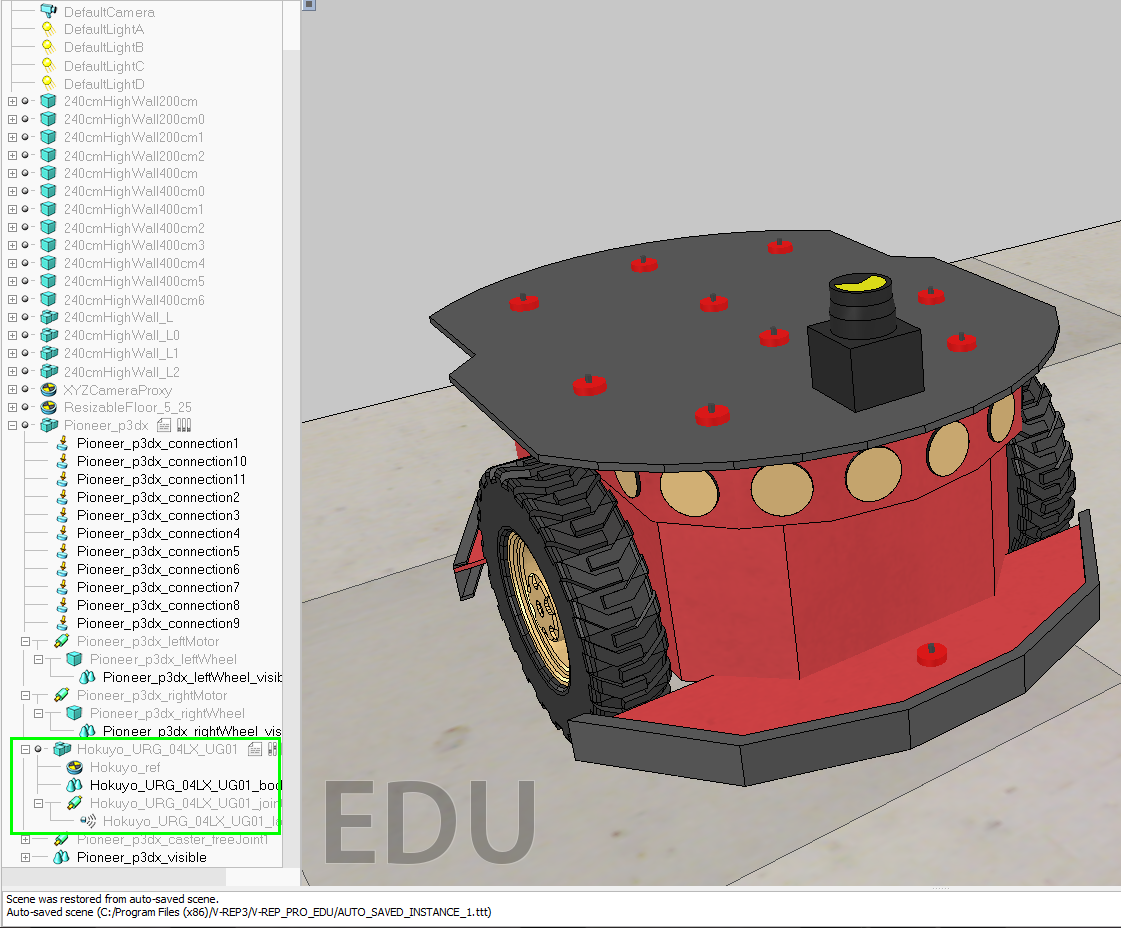
\includegraphics[width=0.7\textwidth]{imagens/insercao_elementos_vrep}
	\caption{Árvore Hierárquica V-Rep}
	\label{fig:arvore-v-rep}
\end{figure}

\paragraph{}
Na figura \ref{fig:arvore-v-rep} também é possível observar a posicionamento do sensor, que terá seu \emph{frame} movimentado na mesma direção, sentido e velocidade da movimentação do \emph{frame} do robô, o objeto pai.




\chapter{Resultados}
Texto sobre os resultados obtidos, tamanho e organiza\c{c}\~{a}o das informa\c{c}\~{o}es
\chapter{Conclus\~{a}o}
Considera\c{c}\~{o}es finais sobre o trabalho
\appendix
\chapter{Códigos Fonte}

\begin{table}
\caption{Armadillos}
\label{arm:table}
\begin{center}
\begin{tabular}{||l|l||}\hline
Armadillos & are \\\hline
our	   & friends \\\hline
\end{tabular}
\end{center}
\end{table}

\clearpage
\newpage

%\chapter{Figuras}

\vspace*{-3in}

\begin{figure}
\vspace{2.4in}
\caption{Armadillo slaying lawyer.}
\label{arm:fig1}
\end{figure}
\clearpage
\newpage

\begin{figure}
\vspace{2.4in}
\caption{Armadillo eradicating national debt.}
\label{arm:fig2}
\end{figure}
\clearpage
\newpage

%% This defines the bibliography file (main.bib) and the bibliography style.
%% If you want to create a bibliography file by hand, change the contents of
%% this file to a `thebibliography' environment.  For more information 
%% see section 4.3 of the LaTeX manual.

\begin{singlespace}
%\addcontentsline{toc}{section}{Refer\^{e}ncias Bibliogr\'{a}ficas}
%\bibliography{main}
%\bibliography{ieee}
\bibliography{reference_bibtex}
%\bibliography{ieee_2}
\bibliographystyle{plain}
\end{singlespace}

\end{document}

